    \documentclass[a4paper]{article}
\usepackage{blindtext}
\usepackage[T1]{fontenc}
\usepackage{lmodern}
\usepackage[utf8]{inputenc}
\usepackage[unicode]{hyperref}
\usepackage{amsfonts}
\usepackage{amsmath}
\usepackage{graphicx}
\usepackage{outlines}
\usepackage{pdfpages}
\usepackage{geometry}
\usepackage{svg}
\usepackage{mathtools}
\usepackage{enumitem}
\usepackage{amsthm}
\usepackage{titlesec}
\usepackage{float}
\usepackage{enumitem}
\usepackage{array}
\usepackage{color, colortbl}
\usepackage{graphicx}
\usepackage{subcaption}
\usepackage{mwe}
\usepackage[ruled,vlined]{algorithm2e}
\usepackage{biblatex}
\usepackage{listings}
\addbibresource{p.bib}


\newcommand*{\naturalNumbers}{\mathbb{N}}%

\title{Hate speech classification}
\author{Paweł Flis, Karol Krupa, Rafał Chabasiński}
\date{June 2022}

\begin{document}
\maketitle

\section{Introduction}
Social media platforms such as Facebook, Twitter, Instagram and YouTube are experiencing a continuous growth in number of users. In recent years, partially due to COVID-19 pandemic even older generations turned to those platforms as a way to experience wider range of human interactions. Along with all the advantages social media brings, there are number of hazards related to harmful actions of some of its users encouraged by their perceived anonymity.
\par
Especially recently hate speech has been under the scope of investigation to make the internet a safe and welcoming space for everyone. This topic garnered scientific attention due to the potential of applying machine learning for hate speech recognition, which would in turn help counteract cyberbullying. Although the very idea of using automatic censors is highly questionable their counselling can be of invaluable aid. In this case the hate speech detector accuracy is of the essence as too rigorous model could severely affect freedom of expression while high-tolerance one would maintain unsafe environments.
\section{Literature analysis}
Number of Natural Language Processing in conjunction with Deep Learning solutions have been proposed during the years, however majority of these solutions requires great amount of labelled data, which has to be manually labeled by a human, which eventually limits the cognitive capabilities of the model. It is also really hard to identify semantic nuances which often decide on the overall sentiment. There have been attempts to tackle the problem using statistical models such as n-grams, SVM or Logistic Regression. These methods require vector as an input, so the corpus of text has to be converted earlier - this is commonly done using methods such as word2vec encoder using semantic similarity of words or doc2vec for entire sentences.
\par
The task at hand is hate speech detection in polish twitter data. Direct solution to the same problem were presented during PolEval2019~\cite{poleval}. At a time statistical models such as SVM with tokenization or even Deep Learning solutions such as LSTM were able to achieve only minor improvements over baseline classifier which always predicts most common class.
\par
Bidirectional Encoder Representations from Transformers model has shown a great prowess in various NLP tasks, in many cases outperforming its predecessors.
Mozafari et al.~\cite{paper} proposed a semi-supervised solution based on pre-trained BERT model with broad contextual knowledge and using transfer learning to fine tune a model on labelled samples from target domain of hate speech. 
\par
This approach considers two variants of BERT networks. $BERT_{base}$ having 12 layers and 110 million parameters and $BERT_{large}$ having double the layers and triple the parameters. The output is a sentence representation in a 768-dimensional vector, which is an input to domain specific classifier.
\par
In paper number of fine-tuning approaches are presented:
\begin{enumerate}
    \item \textbf{BERT based fine-tuning} \\
    $BERT_{base}$ model with one fully connected layer at the top and softmax activation function with no hidden layers.
    \item \textbf{Insert nonlinear layers} \\
    $BERT_{base}$ model with multilayer perceptron with two hidden layers at the top level.
    \item \textbf{Insert Bi-LSTM layer} \\
    $BERT_{base}$ model with Bi-LSTM recurrent neural network and one fully connected layer on the output.
    \item \textbf{Insert CNN layer} \\
    Output of each transformer from $BERT_{base}$ is concatenated to produce a matrix that is an input to CNN, later max pooling is performed and output is deduced using one fully connected layer once agian.
\end{enumerate}
\par
The authors performed data pre-processing to make the text input data more suitable for BERT model - emoticons were changed into <tags>, multiple word hashtags were separated and everything has been turned into lowercase. It is important to notice, that by doing that some relevant information may be lost, however we trust that it is a calculated decision and it is of benefit to used BERT model.
\par
Version with CNN layer proved to perform the best across all metrics (Precision, Recalll, F1-score). It outperformed other solutions designed for the very same datasets used in  ~\cite{ref1}~\cite{ref2}~\cite{ref3}. It is worth noting that BERT with nonlinear layers performed surprisingly poorly(much worse than with no hidden layers) on dataset with samples labelled as Hate[1430] Offensive[19190] Neither[4163] so dataset heavily biased towards 'just' offensive content.

\newpage
\section{Exploratory data analysis}
We've acquired our data from \url{http://2019.poleval.pl/tasks/task6}. \\
Training data was taken from section Task description, Task 6-2: Type of harmfulness. Test data was available in the later section 'Test data'. \\

The data row comprised of two elements - sentence and its classification to one of three classes. The classes were: 0 (non-harmful), 1 (cyberbullying) and 2 (hate-speech). \\

The condition to distinguish cyberbulling from hate speech was whether the harmful action is addressed towards a private person(s) (cyberbullying), or a public person/entity/large group (hate-speech).

\subsection{Data examples}
\begin{itemize}
    \item non-harmful
        \begin{itemize}
            \item anonymizedaccount anonymizedaccount Zaległości były, ale ważne czy były wezwania do zapłaty z których się klub nie wywiązał.
            \item anonymizedaccount Tym w sejmie też? Banda hipokrytów i złodziei.
        \end{itemize}
    \item cyberbullying
        \begin{itemize}
            \item anonymizedaccount anonymizedaccount Czas pokaże kto jest kim, mącicielu, szkodniku, haha do gazu haha
            \item anonymizedaccount anonymizedaccount anonymizedaccount Pis mial być inny, jesteś idiotą
        \end{itemize}
    \item hate-speech
        \begin{itemize}
            \item RT anonymizedaccount anonymizedaccount Pasujecie do siebie antypolskie kanalie.
            \item anonymizedaccount Pierwszy priorytet zadowolić Jarkacza, drugi priorytet ssać kasę wszystkimi otworami,  mają rozdwojenie jaźni
        \end{itemize}
\end{itemize}

We can see that subjects are anonymized and are easily recognizable, which will be helpful for our algorithms.

\newpage
\subsection{Label data split}
\begin{figure}[h]
\centering
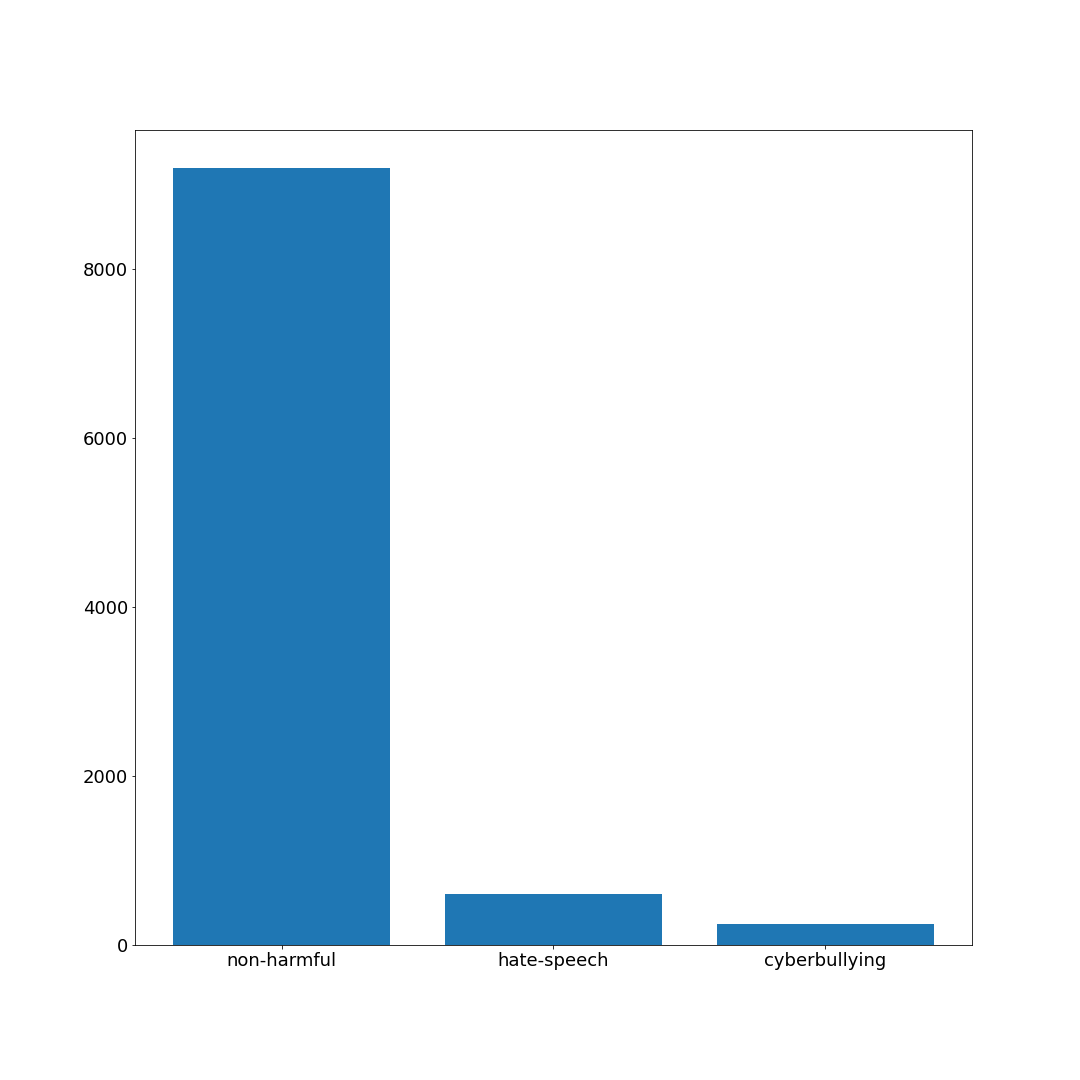
\includegraphics[width=\textwidth]{plots/tags_bar_plot.png}
\caption{Labels distribution.}
\label{fig:labels_distribution}
\end{figure}

In \ref{fig:labels_distribution} we can see that distribution of classes in the dataset is very unbalanced. We'll have to consider that when creating our algorithm, by e.g.
\begin{itemize}
    \item shrinking bigger data sets to the smallest one
    \item applying bigger weights to smaller datasets
\end{itemize}


\newpage
\subsection{Data attributes}

\begin{figure}[H]
\centering
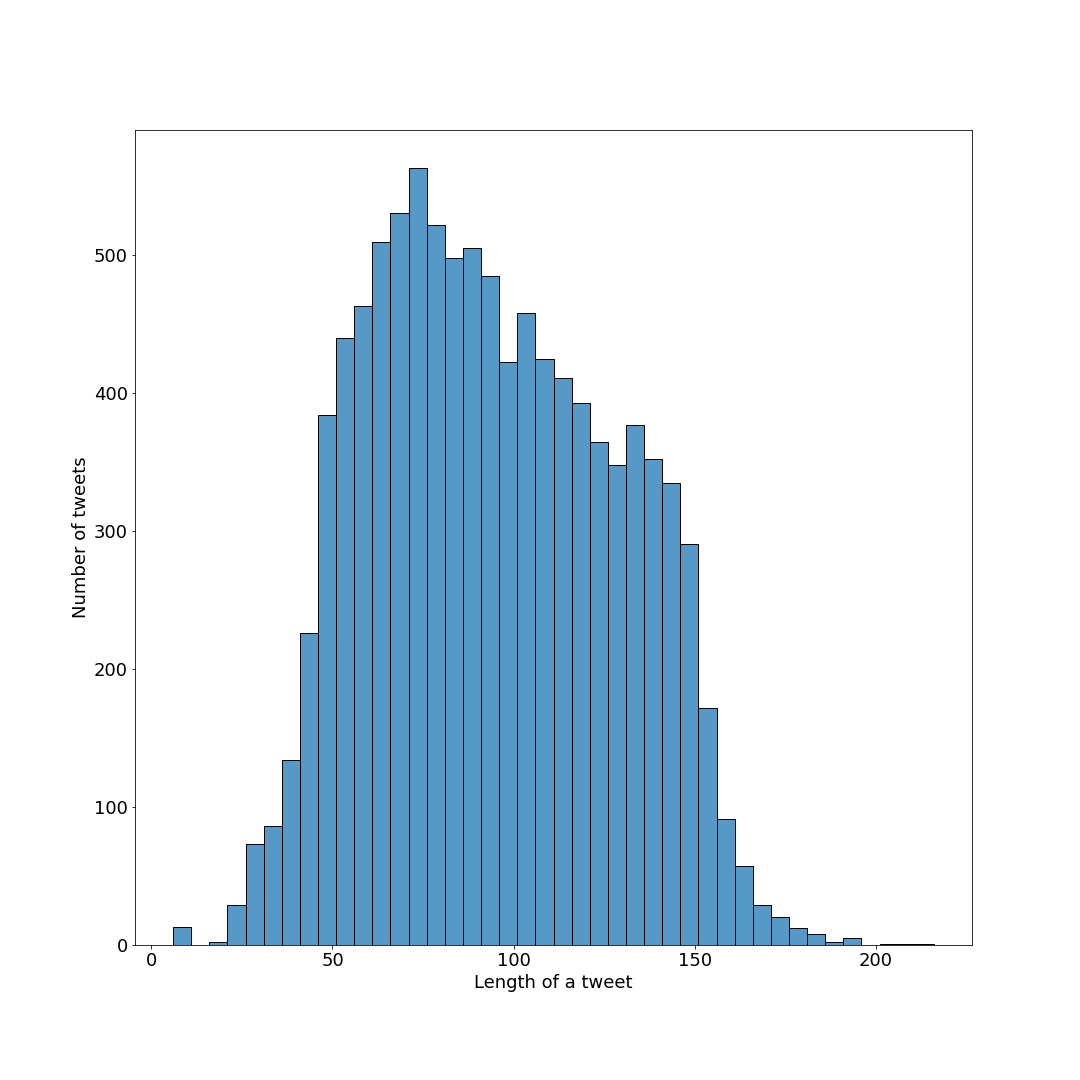
\includegraphics[width=\textwidth]{plots/tweet_lengths_plot.png}
\caption{Tweets lengths (i.e number of characters in a tweet).}
\label{fig:tweet_lengths_histogram}
\end{figure}

\begin{figure}[H]
\centering
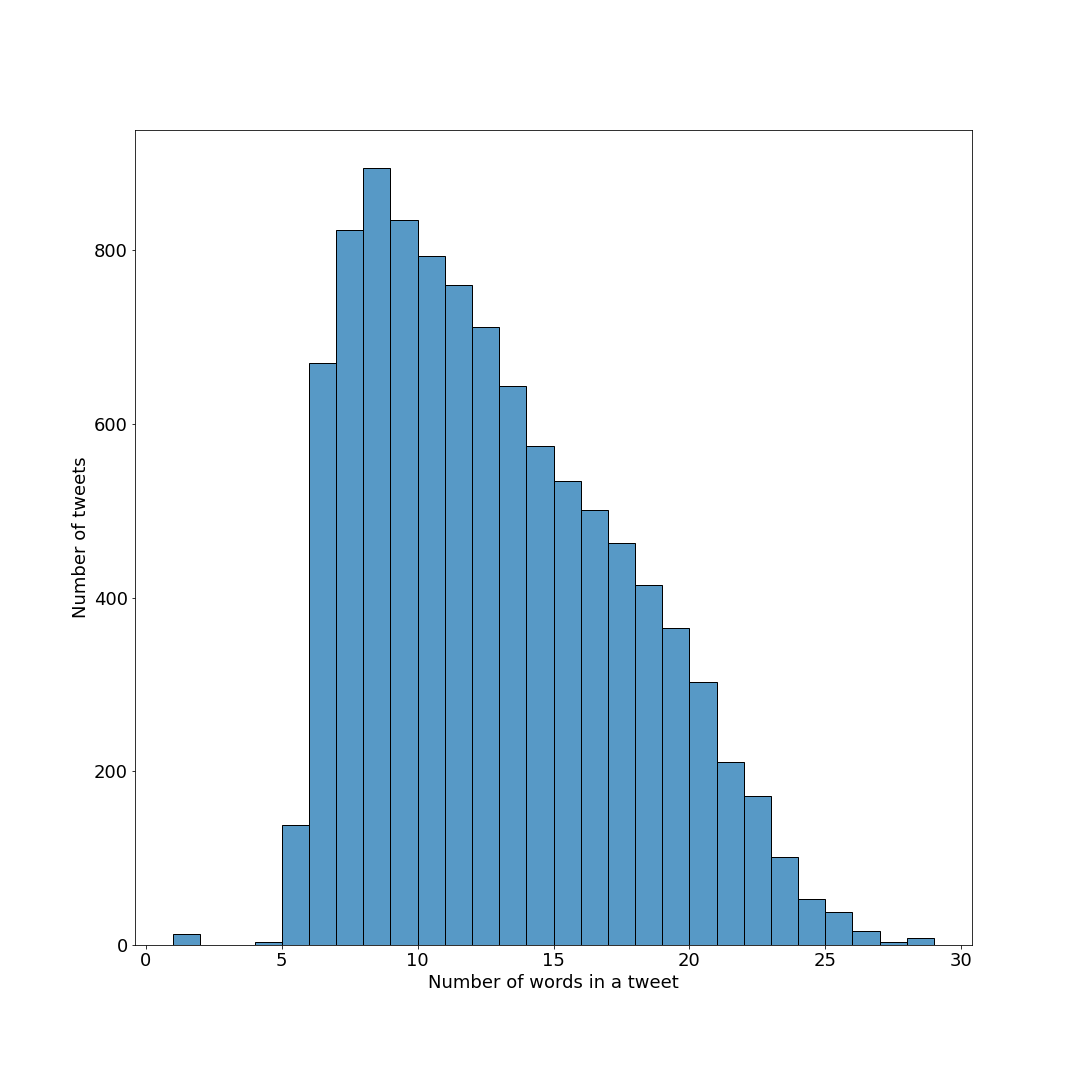
\includegraphics[width=\textwidth]{plots/tweet_word_counts_plot.png}
\caption{Tweets word counts.}
\label{fig:word_counts_histogram}
\end{figure}

We created histograms for length of a tweet and number of words in a tweet. \\
In both graphs (\ref{fig:tweet_lengths_histogram} and \ref{fig:word_counts_histogram}) we can see some outliers in the data. In order to simplify our task and make our solution more reliable we should consider removing them.


\begin{figure}[H]
\centering
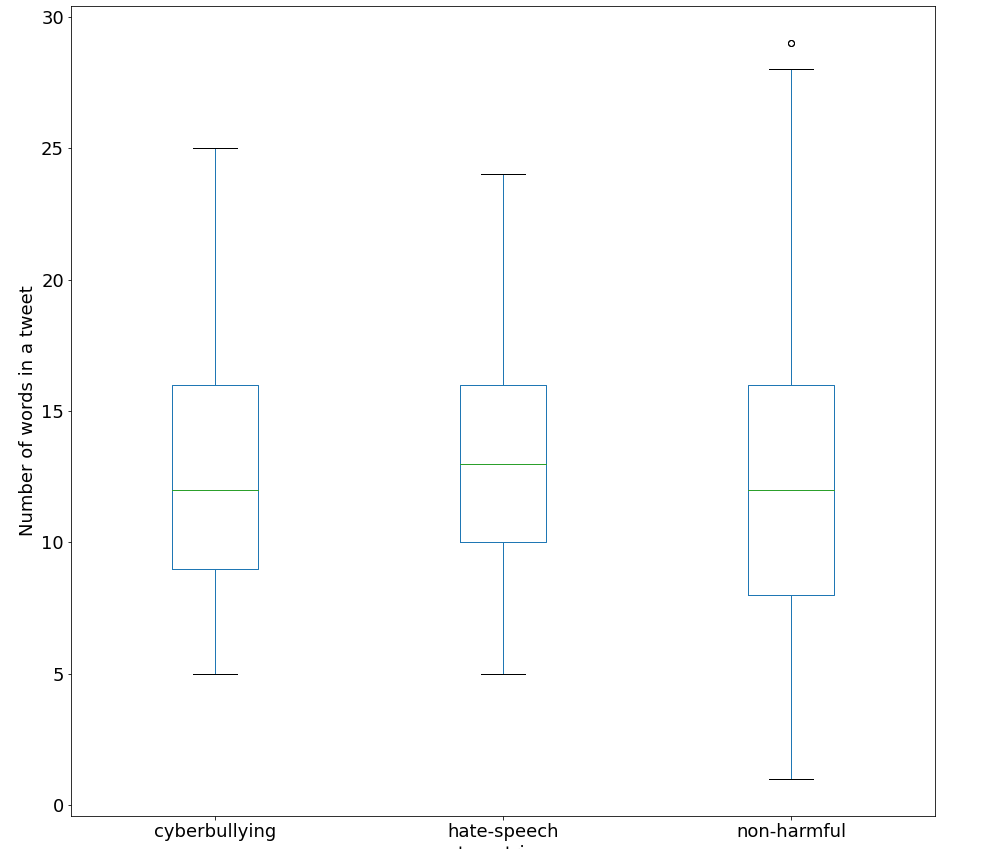
\includegraphics[width=\textwidth]{plots/tweet_word_counts_box_plot.png}
\caption{Tweets word counts box plot for different labels.}
\label{fig:box_plot}
\end{figure}

We've created boxplots for number of words in a tweet for all classes \ref{fig:box_plot}. \\
Unfortunately, different labels have quite similar expected values for number of words, so this statistic most likely won't help us.

\subsection{Word cloud}

\begin{figure}[H]
\centering
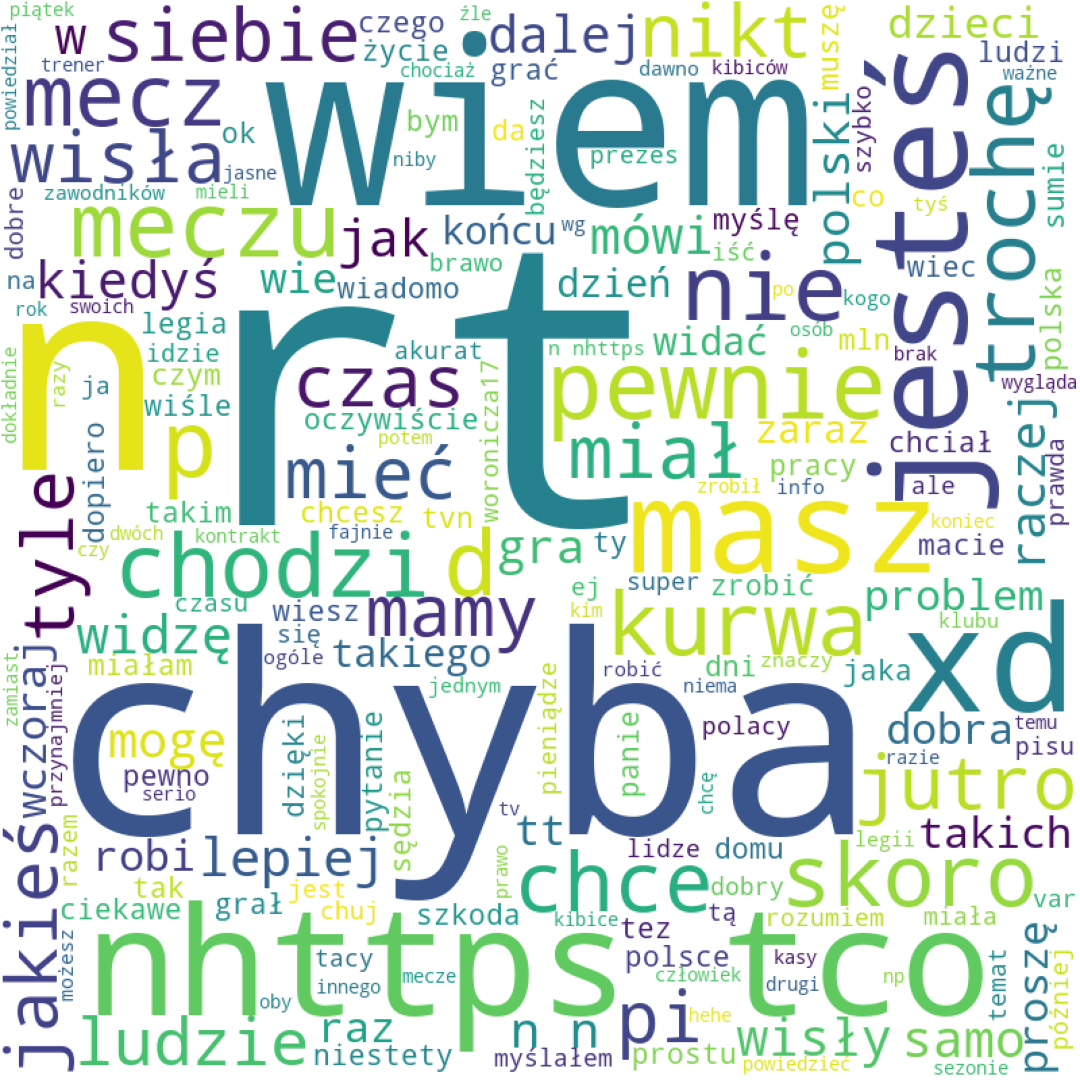
\includegraphics[width=\textwidth]{plots/word_cloud.png}
\caption{Word cloud.}
\label{fig:word_cloud}
\end{figure}

In \ref{fig:word_cloud} we can see that the most important topics in our dataset are football and politics. There are also some curse words which may help distinguish hate speech. \\ Some one letter words and specific stop words can be distinguished, so removing them might further help us remove noise from the data.

\newpage
\section{Solution concept}

Preparing our solution to the problem is to prepare a program that, given an expression written by a human, returns a result of 1 if the statement is hate-filled and 0 otherwise. 

In order to perform this task as well as possible, we need to:
\begin{enumerate}
    \item Properly transfer expressions and sentences into a form understandable by a computer - that is, vectorize them using an appropriate tokenizer. 
    \item Model the language and its internal dependencies using certain language models.
    \item Train the language models for our task, which is hate speech recognition.
\end{enumerate}

The first two steps can be solved by choosing a pretrained model. A collection of such models is available at this link \href{https://klejbenchmark.com/leaderboard/}{KLEJ-Benchmark}.
The first two steps are strongly related, since the trained model has been trained for selected embeddings and is unlikely to work for others.

An example model from the list above is HerBERT \cite{mroczkowski-etal-2021-herbert} and XLM-RoBERTa \cite{dadas2020pretraining}. Both score very high on the CBD task \cite{ptaszynski2019results}, which is the task we solve. For this reason, we decided to select pre-trained models and then retrain them for our purposes.
In addition, for the second model, the authors provided scripts that give the ability to train the model to a specific KLEJ-benchmark problem, including the CBD problem. The scripts are available here: \href{https://github.com/sdadas/polish-roberta}{scripts}.

The computations will be done with google cloud graphics cards, on the google collab site. Verification will be done using Precision, Recalll, F1-score metrics.

In addition to this, research will be conducted on simpler models such as decision trees, SVMs, and naive Bayes. Various embedders such as count vectorizer, tfidf and spacy embedders will be tested. 

\newpage
\section{Solution}

\subsection{Data preprocessing}

During the development of the solution, a significant element was the proper preprocessing of the data. The proposed solution performs three-stage data processing:

\begin{enumerate}
    \item Optional stemming of words in sentences using \href{https://github.com/Tutanchamon/pl_stemmer/blob/master/pl_stemmer.py}{stemmer}.
    \item Main sentence preprocessing module consisting of:
    \begin{enumerate}
        \item Lowering letters
        \item Unidecoding
        \item Removing @anonymized\_account phrase, dots and commas
    \end{enumerate}
    \item Removing stopwords. List of stopwords is taken from \href{https://github.com/bieli/stopwords/blob/master/polish.stopwords.txt}{there}.
\end{enumerate}

The reprocessed datasets are stored in the solution repository in folder data in files: test\_preprocessed.tsv, train\_preprocessed.tsv, test\_preprocessed\_stem.tsv, train\_preprocessed\_stem.tsv.

\subsection{Decision tree}

At the beginning of the preparation of the machine learning solution to the problem posed, we started the tests by building a model closest to the rule-based system. The choice was to build a decision tree based on CountVectorizer with 1 element ngrams. We ran a series of tests in which we examined the effect of tree depth on the results obtained. Results can be seen in figure \ref{fig:decision_tree_height_comparison}. 

\begin{figure}[h]
\centering
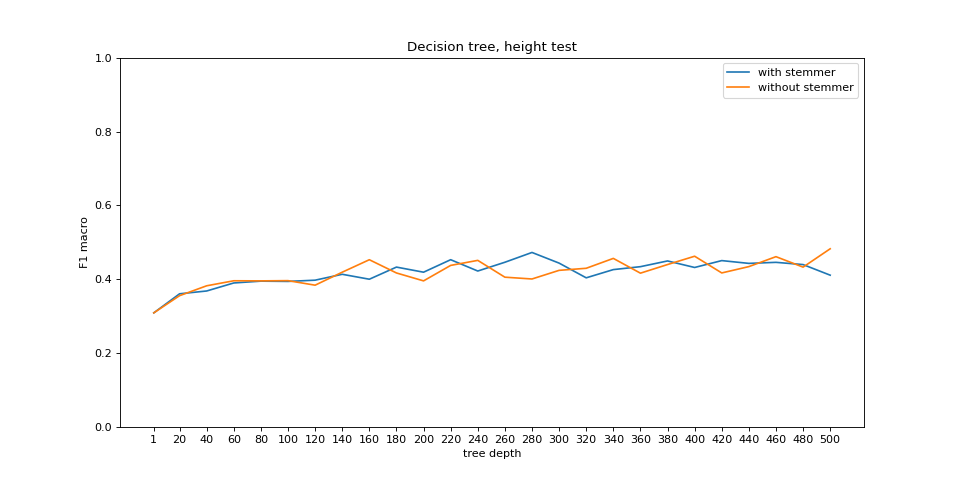
\includegraphics[width=\textwidth]{plots/decision_tree_height_comparison.png}
\caption{Decision tree height comparison}
\label{fig:decision_tree_height_comparison}
\end{figure}

Best obtained result for stemmed and not stemmed data are grouped in the table \ref{tab:decision_tree_hc_results}.

\begin{table}[h]
\centering
\begin{tabular}{|l|l|l|l|l|}
\hline
No. & Stemmed data & Best tree height & F1 macro & F1 micro \\ \hline
1   & true         & 280              & 0.473    & 0.868    \\ \hline
2   & false        & 500              & 0.483    & 0.87     \\ \hline
\end{tabular}
\caption{Decision tree height comparison, results}
\label{tab:decision_tree_hc_results}
\end{table}

The performance of the decision trees increases during the initial phase of increasing the tree height, however, the fluctuations are quite high thereafter. This does not change the fact that good results have been achieved with the decision tree. However, it should be kept in mind that this solution is very dependent on the test set and does not take into account the meaning of the words, which can have very negative consequences when the vocabulary changes 


As part of the development of the solution, we have also prepared an illustration showing how the decision making is done for an example tree of height 3. The result is available in figure \ref{fig:example_tree}.

\begin{figure}[h]
\centering
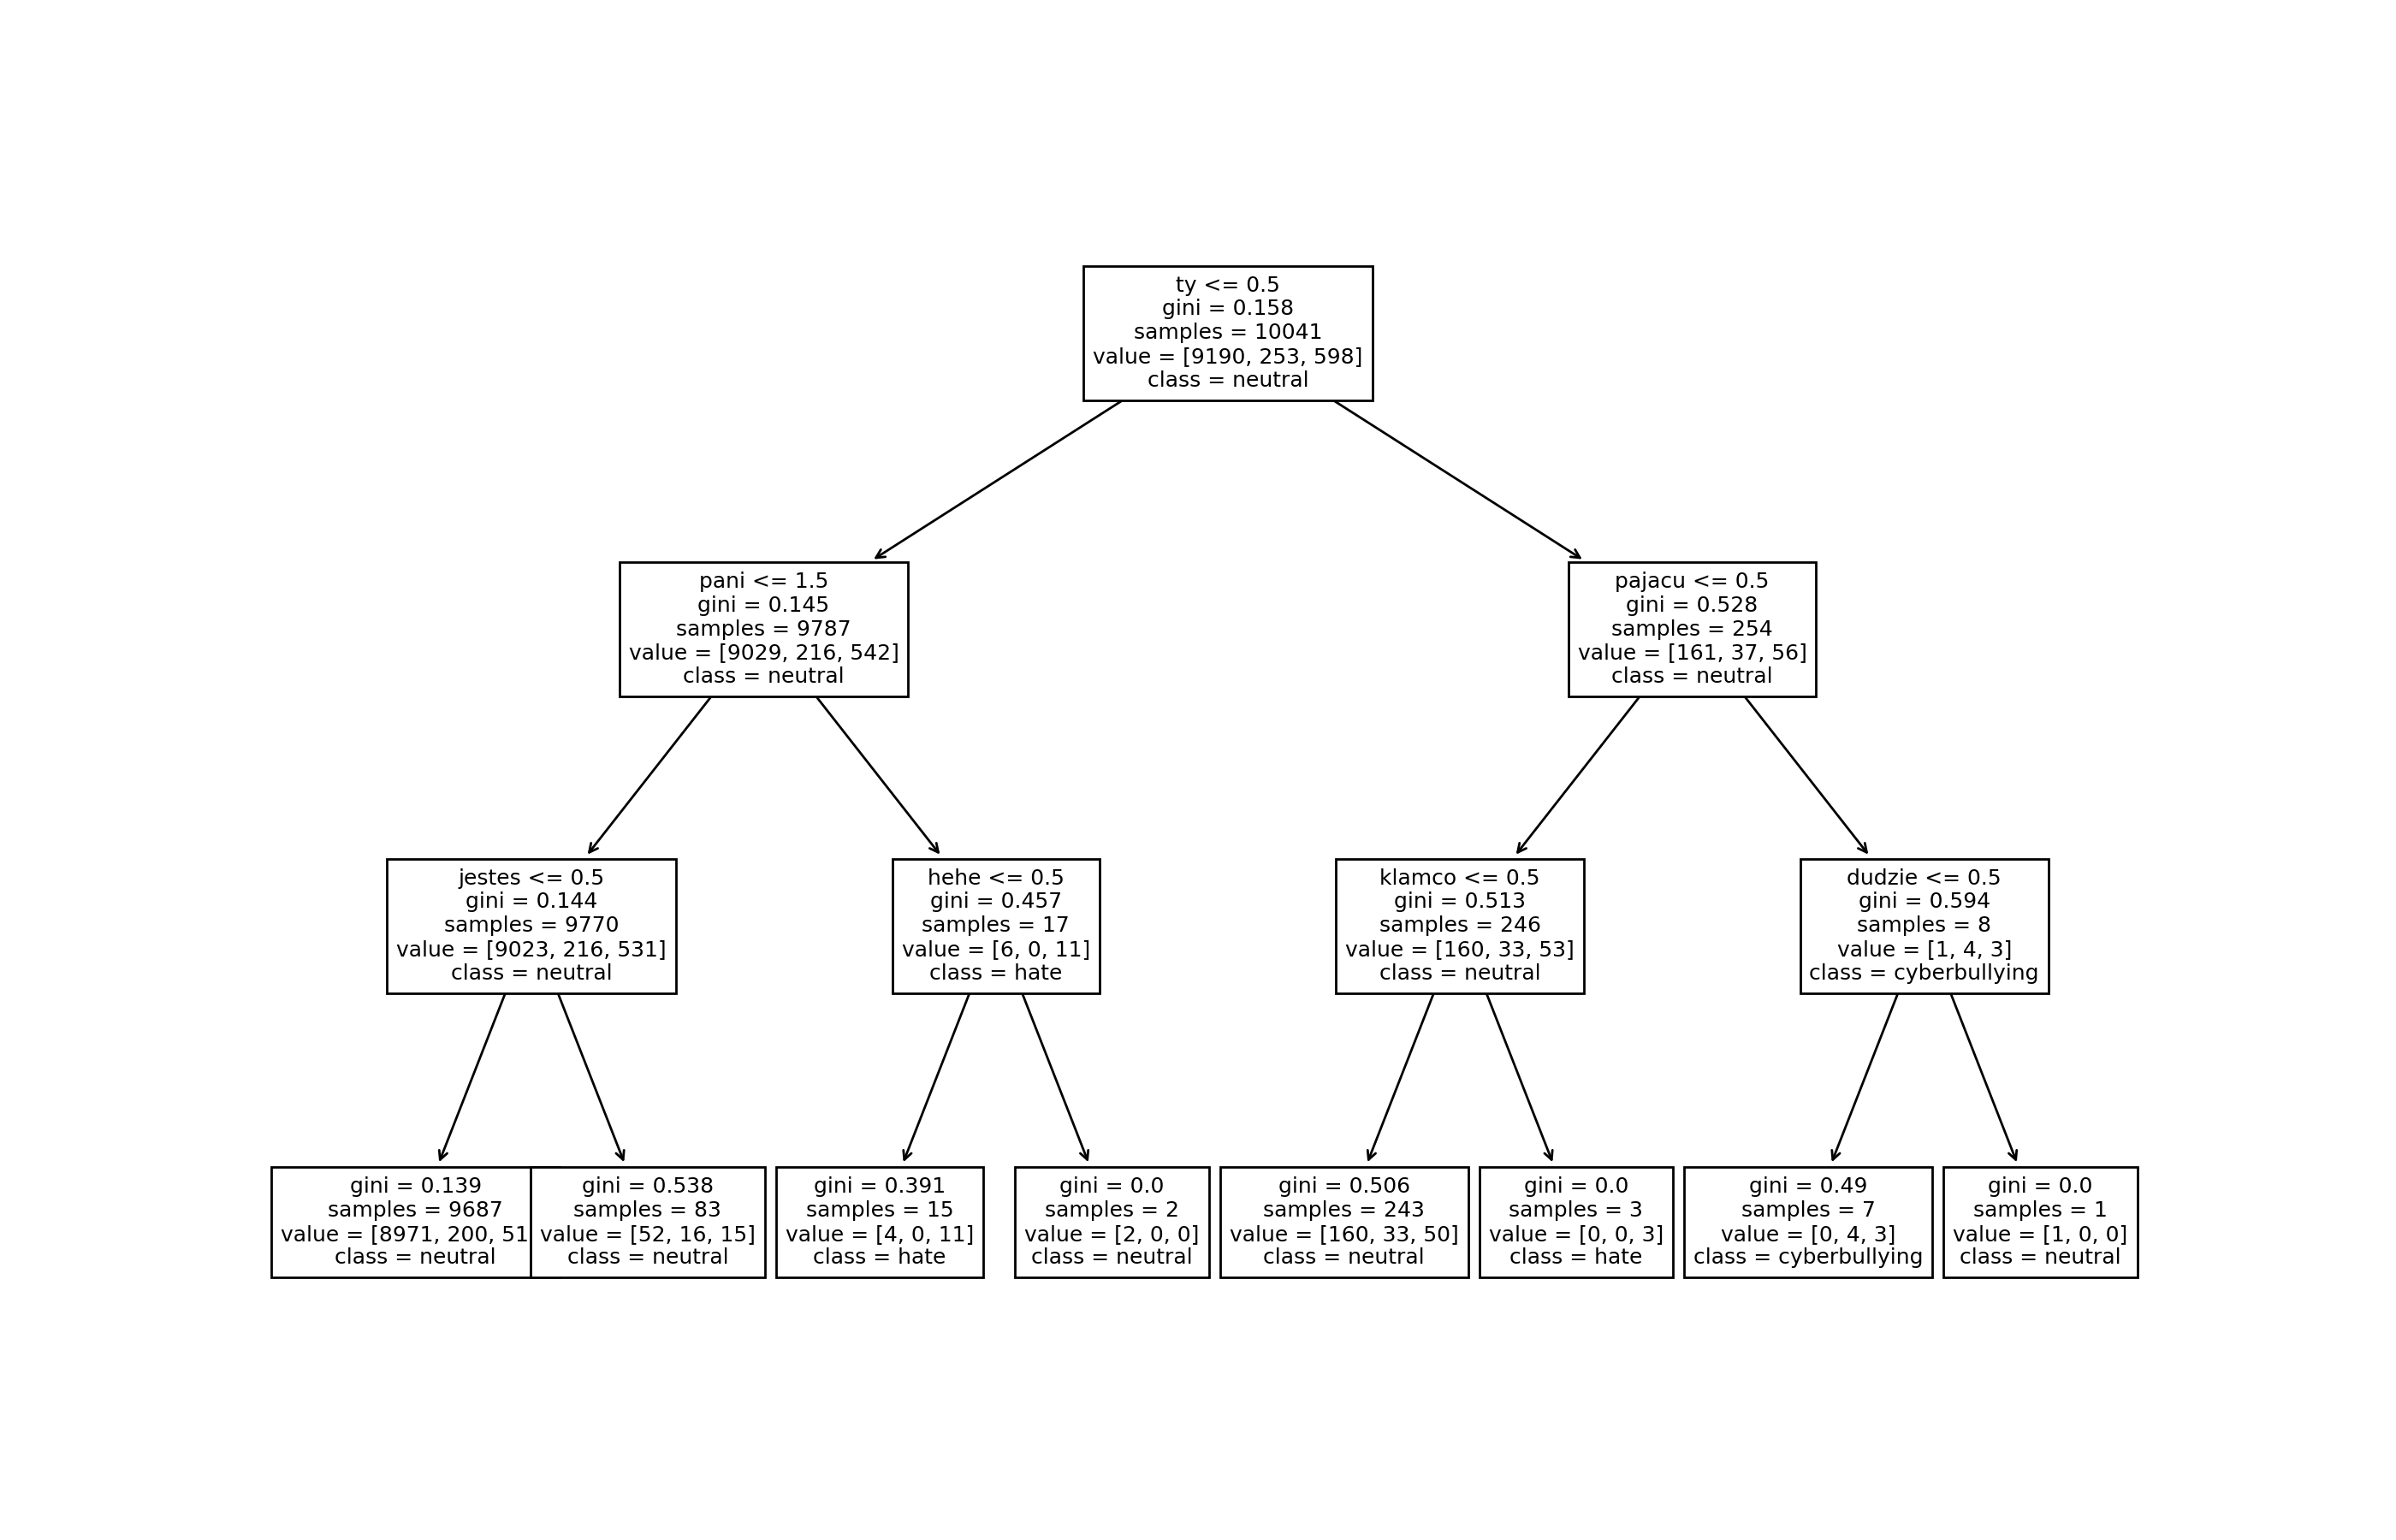
\includegraphics[width=\textwidth]{plots/decision_tree_plot.png}
\caption{Example decision tree with depth = 3 and F1 macro 0.309}
\label{fig:example_tree}
\end{figure}


\subsection{SVM and Naive Bayes}

During the development of the solution, we experimented also with SVM models with three different kernels: RBF, Poly, Linear. In addition, we also considered the Naive Bayes model. To analyze these solutions, we proposed a text vectorizer computed from 1 or 2 element ngrams. Then the 5 or 10\% most significant elements were selected. Moreover, each experiment was performed twice - for the set with and without the applied stemmer. The collected results can be found in the table \ref{tab:simple_results}.


\begin{table}[h]
\centering
\begin{tabular}{llllllll}
\hline
\multicolumn{1}{|l|}{No.} & \multicolumn{1}{l|}{model}       & \multicolumn{1}{l|}{ngram} & \multicolumn{1}{l|}{selector\_percentile} & \multicolumn{1}{l|}{F1 macro (S)} & \multicolumn{1}{l|}{F1 micro (S)} & \multicolumn{1}{l|}{F1 macro} & \multicolumn{1}{l|}{F1 micro} \\ \hline
\multicolumn{1}{|l|}{1}   & \multicolumn{1}{l|}{SVM RBF}     & \multicolumn{1}{l|}{1}     & \multicolumn{1}{l|}{5}                    & \multicolumn{1}{l|}{0.365}        & \multicolumn{1}{l|}{0.873}        & \multicolumn{1}{l|}{0.350}    & \multicolumn{1}{l|}{0.871}    \\ \hline
\multicolumn{1}{|l|}{2}   & \multicolumn{1}{l|}{SVM RBF}     & \multicolumn{1}{l|}{1}     & \multicolumn{1}{l|}{10}                   & \multicolumn{1}{l|}{0.367}        & \multicolumn{1}{l|}{0.864}        & \multicolumn{1}{l|}{0.369}    & \multicolumn{1}{l|}{0.861}    \\ \hline
\multicolumn{1}{|l|}{3}   & \multicolumn{1}{l|}{SVM RBF}     & \multicolumn{1}{l|}{2}     & \multicolumn{1}{l|}{5}                    & \multicolumn{1}{l|}{0.399}        & \multicolumn{1}{l|}{0.869}        & \multicolumn{1}{l|}{0.403}    & \multicolumn{1}{l|}{0.871}    \\ \hline
\multicolumn{1}{|l|}{4}   & \multicolumn{1}{l|}{SVM RBF}     & \multicolumn{1}{l|}{2}     & \multicolumn{1}{l|}{10}                   & \multicolumn{1}{l|}{0.351}        & \multicolumn{1}{l|}{0.864}        & \multicolumn{1}{l|}{0.356}    & \multicolumn{1}{l|}{0.866}    \\ \hline
\multicolumn{1}{|l|}{5}   & \multicolumn{1}{l|}{SVM Poly}    & \multicolumn{1}{l|}{1}     & \multicolumn{1}{l|}{5}                    & \multicolumn{1}{l|}{0.398}        & \multicolumn{1}{l|}{0.875}        & \multicolumn{1}{l|}{0.366}    & \multicolumn{1}{l|}{0.873}    \\ \hline
\multicolumn{1}{|l|}{6}   & \multicolumn{1}{l|}{SVM Poly}    & \multicolumn{1}{l|}{1}     & \multicolumn{1}{l|}{10}                   & \multicolumn{1}{l|}{0.322}        & \multicolumn{1}{l|}{0.867}        & \multicolumn{1}{l|}{0.321}    & \multicolumn{1}{l|}{0.867}    \\ \hline
\multicolumn{1}{|l|}{7}   & \multicolumn{1}{l|}{SVM Poly}    & \multicolumn{1}{l|}{2}     & \multicolumn{1}{l|}{5}                    & \multicolumn{1}{l|}{0.339}        & \multicolumn{1}{l|}{0.87}         & \multicolumn{1}{l|}{0.339}    & \multicolumn{1}{l|}{0.869}    \\ \hline
\multicolumn{1}{|l|}{8}   & \multicolumn{1}{l|}{SVM Poly}    & \multicolumn{1}{l|}{2}     & \multicolumn{1}{l|}{10}                   & \multicolumn{1}{l|}{0.322}        & \multicolumn{1}{l|}{0.868}        & \multicolumn{1}{l|}{0.322}    & \multicolumn{1}{l|}{0.868}    \\ \hline
\multicolumn{1}{|l|}{\textbf{9}}   & \multicolumn{1}{l|}{\textbf{SVM Linear}}  & \multicolumn{1}{l|}{\textbf{1}}     & \multicolumn{1}{l|}{\textbf{5}}                    & \multicolumn{1}{l|}{\textbf{0.409}}        & \multicolumn{1}{l|}{\textbf{0.877}}        & \multicolumn{1}{l|}{\textbf{0.375}}    & \multicolumn{1}{l|}{\textbf{0.874}}    \\ \hline
\multicolumn{1}{|l|}{10}  & \multicolumn{1}{l|}{SVM Linear}  & \multicolumn{1}{l|}{1}     & \multicolumn{1}{l|}{10}                   & \multicolumn{1}{l|}{0.379}        & \multicolumn{1}{l|}{0.871}        & \multicolumn{1}{l|}{0.357}    & \multicolumn{1}{l|}{0.868}    \\ \hline
\multicolumn{1}{|l|}{11}  & \multicolumn{1}{l|}{SVM Linear}  & \multicolumn{1}{l|}{2}     & \multicolumn{1}{l|}{5}                    & \multicolumn{1}{l|}{0.389}        & \multicolumn{1}{l|}{0.872}        & \multicolumn{1}{l|}{0.389}    & \multicolumn{1}{l|}{0.872}    \\ \hline
\multicolumn{1}{|l|}{12}  & \multicolumn{1}{l|}{SVM Linear}  & \multicolumn{1}{l|}{2}     & \multicolumn{1}{l|}{10}                   & \multicolumn{1}{l|}{0.353}        & \multicolumn{1}{l|}{0.869}        & \multicolumn{1}{l|}{0.365}    & \multicolumn{1}{l|}{0.871}    \\ \hline
\multicolumn{1}{|l|}{13}  & \multicolumn{1}{l|}{Naive Bayes} & \multicolumn{1}{l|}{1}     & \multicolumn{1}{l|}{5}                    & \multicolumn{1}{l|}{0.322}        & \multicolumn{1}{l|}{0.868}        & \multicolumn{1}{l|}{0.322}    & \multicolumn{1}{l|}{0.868}    \\ \hline
\multicolumn{1}{|l|}{14}  & \multicolumn{1}{l|}{Naive Bayes} & \multicolumn{1}{l|}{1}     & \multicolumn{1}{l|}{10}                   & \multicolumn{1}{l|}{0.344}        & \multicolumn{1}{l|}{0.87}         & \multicolumn{1}{l|}{0.349}    & \multicolumn{1}{l|}{0.87}     \\ \hline
\multicolumn{1}{|l|}{15}  & \multicolumn{1}{l|}{Naive Bayes} & \multicolumn{1}{l|}{2}     & \multicolumn{1}{l|}{5}                    & \multicolumn{1}{l|}{0.322}        & \multicolumn{1}{l|}{0.868}        & \multicolumn{1}{l|}{0.322}    & \multicolumn{1}{l|}{0.868}    \\ \hline
\multicolumn{1}{|l|}{16}  & \multicolumn{1}{l|}{Naive Bayes} & \multicolumn{1}{l|}{2}     & \multicolumn{1}{l|}{10}                   & \multicolumn{1}{l|}{0.364}        & \multicolumn{1}{l|}{0.87}         & \multicolumn{1}{l|}{0.364}    & \multicolumn{1}{l|}{0.87}     \\ \hline
                          &                                  &                            &                                           &                                   &                                   &                               &                              
\end{tabular}
\caption{Different SVM and Naive Bayes settings, results, S - stemmed data}
\label{tab:simple_results}
\end{table}

It turns out that Linear SVM using 1 element grams and a 5\% selector on the data with the stemmer applied, turned out to be the best solution from this set. In addition, it can be inferred from the table that only in five cases we obtained an improvement in performance after using stemmer. These are the rows 1, 5, 6, 9, 10.


\subsection{Multilayer perceptron}

The next stage in the development of our solution was to prepare an MLP network with a structure consisting of the following parts:

\begin{itemize}
    \item Linear layer of size input\_size x 200
    \item Dropout layer 0.2
    \item ReLU
    \item Linear layer of size 200 x 50
    \item Dropout layer 0.2
    \item ReLU
    \item Linear layer of size 50 x 3
    \item Softmax
\end{itemize}


During the development of the solution, we prepared an environment to train MLPs along with various vectorizers. We tested the following text vectors as part of our testing:


\begin{itemize}
    \item CountVectorizer with ngrams of size 1, with selector 5\%
    \item CountVectorizer with ngrams of size 2, with selector 5\%
    \item TfidfVectorizer
    \item Spacy pl\_core\_news\_md vectorizer
    \item Spacy pl\_core\_news\_lg vectorizer
\end{itemize}

Each of these tests was performed on stemmed data and without applied stemmer. Each test was run with the Adam optimizer, with an initial learning rate of 1e-4, at 20 epochs, with the CrossEntropy loss function. Training data were reported with batches of size 10. We also implemented a custom subsampler that rejects 80\% of sentences with a label 0 (neutral sentence) - this operation was needed, otherwise the network learned to predict only one class. Also, in the beginning of every experiment random seed was set to same value (1).

The collected test results are shown in the table below.

\begin{table}[h]
\centering
\begin{tabular}{|l|l|l|l|l|l|}
\hline
No. & Vectorizer                             & F1 macro (S) & F1 micro (S) & F1 macro & F1 micro \\ \hline
1   & CountVectorizer, ngram=1, percentile=5 & 0.472        & 0.874        & 0.485    & 0.876    \\ \hline
2   & CountVectorizer, ngram=2, percentile=5 & 0.441        & 0.874        & 0.427    & 0.877    \\ \hline
3   & \textbf{Tfidf}                                  & \textbf{0.481}        & \textbf{0.815}        & \textbf{0.500}    & \textbf{0.828}    \\ \hline
4   & Spacy, pl\_core\_news\_md              & 0.438        & 0.816        & 0.430    & 0.787    \\ \hline
5   & Spacy, pl\_core\_news\_lg              & 0.435        & 0.800        & 0.436    & 0.803    \\ \hline
\end{tabular}
\caption{MLP with different vectorizers, results. S - stemmed data, results for best F1 macro score epoch}
\label{tab:mlp_results}
\end{table}

The best solution turned out to be the one using the tfidf vectorizer on the data without the stemmer applied.

The figure \ref{fig:mlp_training} shows the training processes for each experiment.  

\begin{figure}[h]
\centering
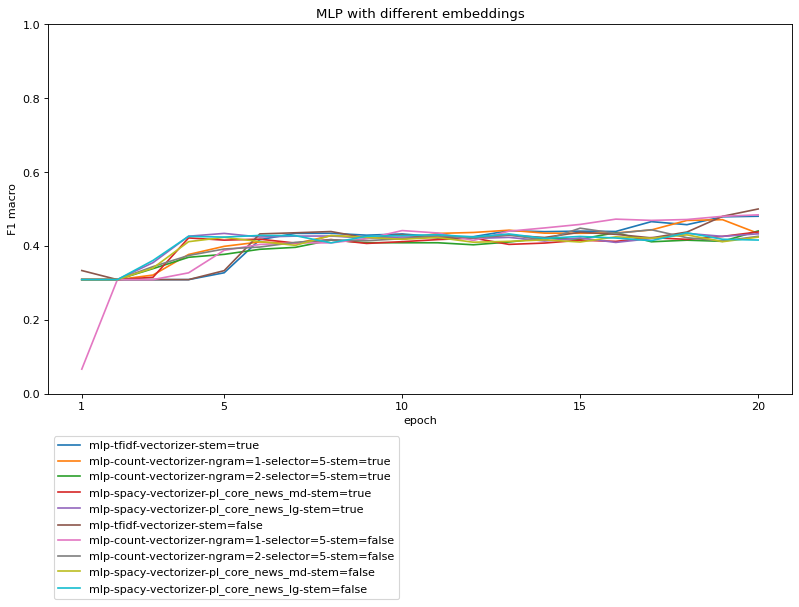
\includegraphics[width=\textwidth]{plots/mlp_with_different_embeddings_comparison.png}
\caption{MLP training processes}
\label{fig:mlp_training}
\end{figure}

One can see on the graph that the training process varies between methods up to about 5 epochs. After that, the process is similar, but the differences in F1 macro statistics are about a few percentage points.

\subsection{Deep learning}

To solve the task using deep learning methods, we used RoBERTa deep machine learning models along with scripts prepared to train them for the KLEJ benchmark prepared by Allegro. The available scripts are \href{https://github.com/sdadas/polish-roberta}{here}. 

During the development of the solution, we used the Collab Pro environment (Google's computing cloud) and the Tesla graphics card that was assigned to us there.

Solution preparation consisted of:
\begin{enumerate}
    \item Prepare the training and testing collection for the CBD task format from the scripts described above. Their Internet hate detection task involved distinguishing between neutral and hate speech. In our case, we have 3 classes: hate, cyber-bullying, and neutral. Moreover, the sets for this task appear in two files: tags and text. Obtaining the intended format required combining these files in tag tab text format.
    \item KLEJ benchmark script modification. The Task CBD described above had 2 categories and was not set up for post-training testing. Because of this, it required code modification. The modified tests.py file is available in the solution repository.
    \item Downloading models on Google Collab.
    \item Beginning model training.
    \item Generating labels for test data.
    \item Running evaluating \href{http://2019.poleval.pl/tasks/task6}{script}.
\end{enumerate}

We tested two models while conducting the experiments. The first one is RoBERTa-large-v2, a model trained on a corpus of about 200GB of data. When training this model, we used the following python script call:

python run\_tasks.py --arch roberta\_large --model\_dir roberta\_large --train-epochs 2 --tasks KLEJ-CBD --fp16 True --max-sentences 8 --update-freq 4 --resample 0:1,1:1,2:1

The training process took approximately 320 seconds (2 epochs) on a Tesla P4 16GB.
 
The parameters mean that we used the roberta\_large architecture, the model is in the roberta\_large folder, we want to train the model for 2 epochs, the task we are doing is TASK-CBD, we want to do the calculations with less precision (meaning they will be done faster), the maximum number of sentences in the GPU at one time is 8, the update rate is 4, the input resampling is 1 for class 0 (neutral), 1 for class 1 (cyber-bullying), 1 for class 2 (hate).

Next, we tested the samplings as 1:15:10 and 0.75:5:3. In addition, we tested the performance of the RoBERTa-base model trained on a 20GB body, which is 10x smaller than the RoBERTa-large-v2.

The results obtained can be found in \ref{tab:roberta_results}. 

\begin{table}[h]
\centering
\begin{tabular}{|l|l|l|ll}
\cline{1-3}
                 & micro-average F-score & macro-average F-score &  &  \\ \cline{1-3}
base-075-5-3     & 88.10                 & 57.24                 &  &  \\ \cline{1-3}
large-v2-075-5-3 & 90.00                 & 58.63                 &  &  \\ \cline{1-3}
large-v2-1-1-1   & 90.70                 & 51.48                 &  &  \\ \cline{1-3}
large-v2-1-15-10 & 89.50                 & 54.21                 &  &  \\ \cline{1-3}
\end{tabular}
\caption{RoBERTa with different subsampling methods, results}
\label{tab:roberta_results}
\end{table}

Accuracy was about 90\% in each case, however, it is not very reliable due to the huge advantage of the class of neutral statements.

The results obtained by the script authors were 66.77\% and 74.16\% for the base model and the large model, respectively. Note that the task they performed is significantly simpler, because they only had to distinguish between negative and neutral statements. In our case there is a neutral statement and a negative statement in two variants, which is a more difficult task.

We conducted an experiment using the RoBERT-large-v2 model along with 0:0.75, 1:3 resampling (used by the authors) for a class 2 CBD task. The results obtained are: precision 76.64\%, recall 61.19\%, balanced F-score 68.05\%, accuracy 92.3\%, so much better than in case of solution for 3 class problem.

\newpage
\section{Deployment}
\hspace{0.8cm}
A user interface application was prepared to manually test and use the models we prepared earlier. It was created using gradio library which allows for straight forward creation of ML demos. Previously trained models have been stored in the cache and when you select a model, the corresponding one is loaded. The user can enter any sentence and after pressing the "Submit" button, the classifying method is called and the information whether the sentence is Neutral, Cyber-Bullying or Hate speech is displayed. To run the application first install requirements:
\begin{lstlisting}[language=bash]
  $ pip install -r requirements.txt
\end{lstlisting}
Then run the only cell in python notebook file \emph{deployment.ipynb}. Application will be simultaneously deployed on local http port.
\\
\\
\begin{figure}[h]
\centering
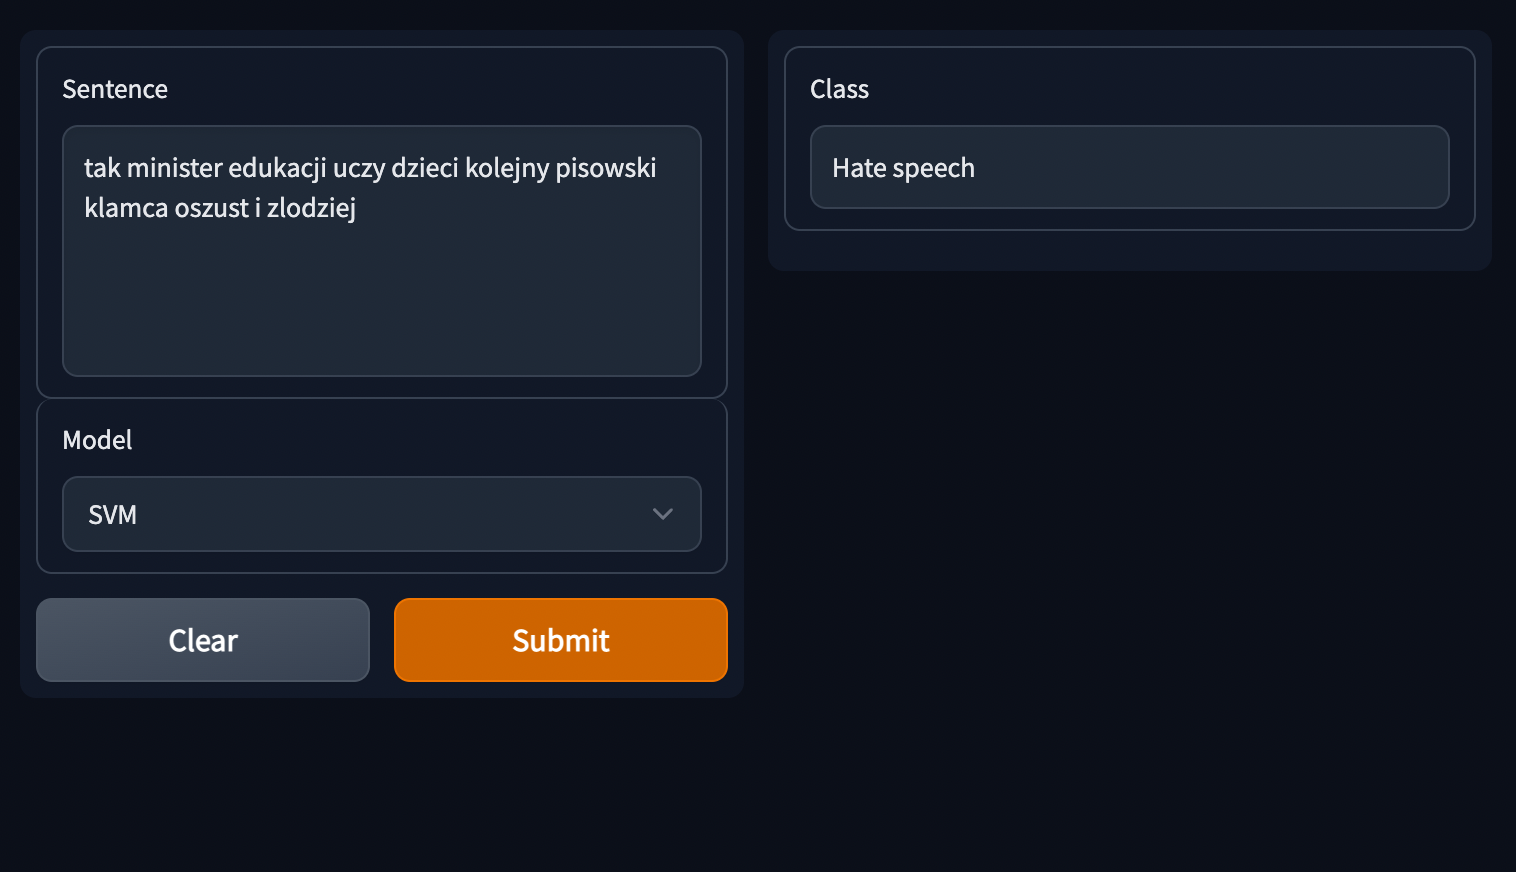
\includegraphics[width=\textwidth]{plots/deployment.png}
\caption{User Interface application}
\label{fig:ui_application}
\end{figure}

\newpage
\section{Summary}

The presented problem of sentence classification in the perspective of neutral/cyberbullying/hate classes consisted in evaluating to which class a given expression belongs. \\
In the literature analysis section, we analysed similar problems (to ours) in the literature. We've also described latest solutions currently used in natural language processing when solving similar tasks. \\

The data prepared for the task was analyzed in these regards: proportion of different classes in the set, lengths of tweets, numbers of characters and the numbers of words. We also checked how the number of words in a tweet depends on the class. Then, an analysis was done on the most frequent words in the text after removing the stopwords. \\

The next stage of the work was to prepare a machine learning solution performing the classification of sentences into netural/cyberbullying/hate classes. First we prepared data for training and testing in both versions - with and without stemming. The first model we tested was a decision tree, which allowed us to build a rule-based system. Here we analyzed the CountVectorizer embedder with 1 element ngrams and checked how trees behave when their size is changed. We performed tests on data with and without stemming. We also prepared visualization of the tree. \\

We then ran tests on SVM and Naive Bayes models. Here we prepared an embedder CountVectorizer with ngrams of 1/2 element and a selector of 5/10\%. We analyzed the behavior of SVM with different kernels with and without stemming data. \\

In the next stage of solution development, we tested the behavior of the Multilayer Perceptron model with CountVectorizer embedders with 1/2 element ngrams + 5/10\% selector, Tfidf, spacy pl\_core\_news\_md and spacy pl\_core\_news\_lg. For MLP training, we also needed to perform subsampling of the training set. \\

In the final stage of development, we tested the RoBERT model using scripts prepared by Allegro for the hate classification task, but based on 2 classes. We adapted the code to our 3 class problem and ran tests for the RoBERTa-large and RoBERTa-base model with different subsampling options for the classes. \\

The problem with CountVectorizer-based embedder solutions is that they depend on a set of training words - word meanings are not taken into account. More complex solutions take this into account. 
Deep learning-based solutions perform much better than models such as SVMs or decision trees, but the process of training them takes much longer, and the environment itself requires GPU hardware. RoBERTa deep learning model is a complex model with many parameters, so it can model language dependencies in an advanced way. For this reason, it performs much better than other solutions. \\

The project was able to present a number of solutions to solve the problem of classifying sentences into netural/cyberbullying/hate classes. Tests of these solutions have been conducted. In the further development of the solution many possibilities arise such as different processing of the input data, testing other embedders and checking the performance of other deep learning models.

\newpage
\printbibliography

\end{document}
 